% Created by tikzDevice version 0.6.2 on 2012-11-28 21:33:54
% !TEX encoding = UTF-8 Unicode
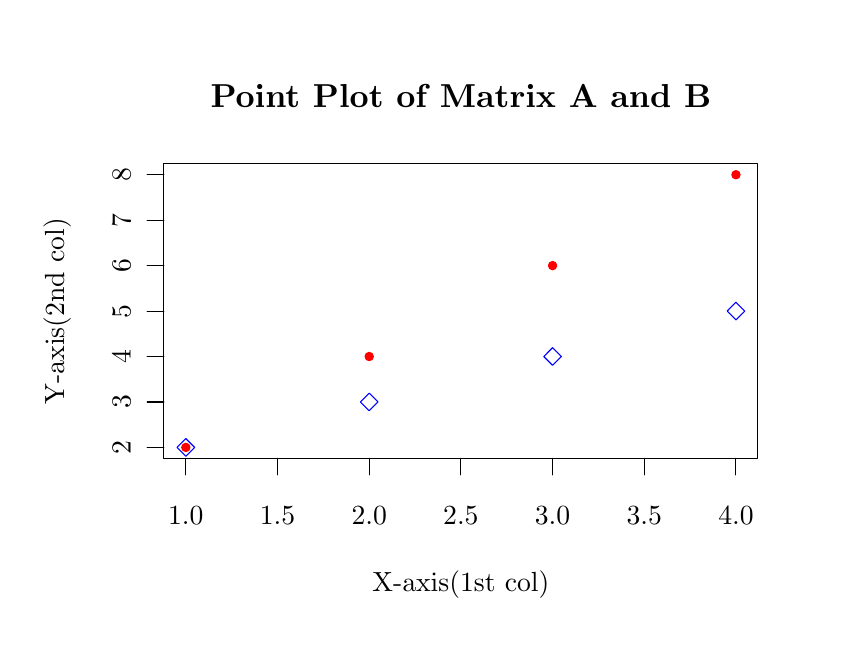
\begin{tikzpicture}[x=1pt,y=1pt]
\definecolor[named]{drawColor}{rgb}{0.00,0.00,0.00}
\definecolor[named]{fillColor}{rgb}{1.00,1.00,1.00}
\fill[color=fillColor,fill opacity=0.00,] (0,0) rectangle (289.08,216.81);
\begin{scope}
\path[clip] ( 49.20, 61.20) rectangle (263.88,167.61);
\definecolor[named]{drawColor}{rgb}{1.00,0.00,0.00}
\definecolor[named]{fillColor}{rgb}{1.00,0.00,0.00}

\draw[color=drawColor,line cap=round,line join=round,fill=fillColor,] ( 57.15, 65.14) circle (  1.50);

\draw[color=drawColor,line cap=round,line join=round,fill=fillColor,] (123.41, 97.98) circle (  1.50);

\draw[color=drawColor,line cap=round,line join=round,fill=fillColor,] (189.67,130.83) circle (  1.50);

\draw[color=drawColor,line cap=round,line join=round,fill=fillColor,] (255.93,163.67) circle (  1.50);
\end{scope}
\begin{scope}
\path[clip] (  0.00,  0.00) rectangle (289.08,216.81);
\definecolor[named]{drawColor}{rgb}{0.00,0.00,0.00}

\draw[color=drawColor,line cap=round,line join=round,fill opacity=0.00,] ( 57.15, 61.20) -- (255.93, 61.20);

\draw[color=drawColor,line cap=round,line join=round,fill opacity=0.00,] ( 57.15, 61.20) -- ( 57.15, 55.20);

\draw[color=drawColor,line cap=round,line join=round,fill opacity=0.00,] ( 90.28, 61.20) -- ( 90.28, 55.20);

\draw[color=drawColor,line cap=round,line join=round,fill opacity=0.00,] (123.41, 61.20) -- (123.41, 55.20);

\draw[color=drawColor,line cap=round,line join=round,fill opacity=0.00,] (156.54, 61.20) -- (156.54, 55.20);

\draw[color=drawColor,line cap=round,line join=round,fill opacity=0.00,] (189.67, 61.20) -- (189.67, 55.20);

\draw[color=drawColor,line cap=round,line join=round,fill opacity=0.00,] (222.80, 61.20) -- (222.80, 55.20);

\draw[color=drawColor,line cap=round,line join=round,fill opacity=0.00,] (255.93, 61.20) -- (255.93, 55.20);

\node[color=drawColor,anchor=base,inner sep=0pt, outer sep=0pt, scale=  1.00] at ( 57.15, 37.20) {1.0};

\node[color=drawColor,anchor=base,inner sep=0pt, outer sep=0pt, scale=  1.00] at ( 90.28, 37.20) {1.5};

\node[color=drawColor,anchor=base,inner sep=0pt, outer sep=0pt, scale=  1.00] at (123.41, 37.20) {2.0};

\node[color=drawColor,anchor=base,inner sep=0pt, outer sep=0pt, scale=  1.00] at (156.54, 37.20) {2.5};

\node[color=drawColor,anchor=base,inner sep=0pt, outer sep=0pt, scale=  1.00] at (189.67, 37.20) {3.0};

\node[color=drawColor,anchor=base,inner sep=0pt, outer sep=0pt, scale=  1.00] at (222.80, 37.20) {3.5};

\node[color=drawColor,anchor=base,inner sep=0pt, outer sep=0pt, scale=  1.00] at (255.93, 37.20) {4.0};

\draw[color=drawColor,line cap=round,line join=round,fill opacity=0.00,] ( 49.20, 65.14) -- ( 49.20,163.67);

\draw[color=drawColor,line cap=round,line join=round,fill opacity=0.00,] ( 49.20, 65.14) -- ( 43.20, 65.14);

\draw[color=drawColor,line cap=round,line join=round,fill opacity=0.00,] ( 49.20, 81.56) -- ( 43.20, 81.56);

\draw[color=drawColor,line cap=round,line join=round,fill opacity=0.00,] ( 49.20, 97.98) -- ( 43.20, 97.98);

\draw[color=drawColor,line cap=round,line join=round,fill opacity=0.00,] ( 49.20,114.40) -- ( 43.20,114.40);

\draw[color=drawColor,line cap=round,line join=round,fill opacity=0.00,] ( 49.20,130.83) -- ( 43.20,130.83);

\draw[color=drawColor,line cap=round,line join=round,fill opacity=0.00,] ( 49.20,147.25) -- ( 43.20,147.25);

\draw[color=drawColor,line cap=round,line join=round,fill opacity=0.00,] ( 49.20,163.67) -- ( 43.20,163.67);

\node[rotate= 90.00,color=drawColor,anchor=base,inner sep=0pt, outer sep=0pt, scale=  1.00] at ( 37.20, 65.14) {2};

\node[rotate= 90.00,color=drawColor,anchor=base,inner sep=0pt, outer sep=0pt, scale=  1.00] at ( 37.20, 81.56) {3};

\node[rotate= 90.00,color=drawColor,anchor=base,inner sep=0pt, outer sep=0pt, scale=  1.00] at ( 37.20, 97.98) {4};

\node[rotate= 90.00,color=drawColor,anchor=base,inner sep=0pt, outer sep=0pt, scale=  1.00] at ( 37.20,114.40) {5};

\node[rotate= 90.00,color=drawColor,anchor=base,inner sep=0pt, outer sep=0pt, scale=  1.00] at ( 37.20,130.83) {6};

\node[rotate= 90.00,color=drawColor,anchor=base,inner sep=0pt, outer sep=0pt, scale=  1.00] at ( 37.20,147.25) {7};

\node[rotate= 90.00,color=drawColor,anchor=base,inner sep=0pt, outer sep=0pt, scale=  1.00] at ( 37.20,163.67) {8};

\draw[color=drawColor,line cap=round,line join=round,fill opacity=0.00,] ( 49.20, 61.20) --
	(263.88, 61.20) --
	(263.88,167.61) --
	( 49.20,167.61) --
	( 49.20, 61.20);
\end{scope}
\begin{scope}
\path[clip] (  0.00,  0.00) rectangle (289.08,216.81);
\definecolor[named]{drawColor}{rgb}{0.00,0.00,0.00}

\node[color=drawColor,anchor=base,inner sep=0pt, outer sep=0pt, scale=  1.20] at (156.54,188.07) {\bfseries Point Plot of Matrix A and B};

\node[color=drawColor,anchor=base,inner sep=0pt, outer sep=0pt, scale=  1.00] at (156.54, 13.20) {X-axis(1st col)};

\node[rotate= 90.00,color=drawColor,anchor=base,inner sep=0pt, outer sep=0pt, scale=  1.00] at ( 13.20,114.41) {Y-axis(2nd col)};
\end{scope}
\begin{scope}
\path[clip] ( 49.20, 61.20) rectangle (263.88,167.61);
\definecolor[named]{drawColor}{rgb}{0.00,0.00,1.00}

\draw[color=drawColor,line cap=round,line join=round,fill opacity=0.00,] ( 53.97, 65.14) --
	( 57.15, 68.32) --
	( 60.33, 65.14) --
	( 57.15, 61.96) --
	( 53.97, 65.14);

\draw[color=drawColor,line cap=round,line join=round,fill opacity=0.00,] (120.23, 81.56) --
	(123.41, 84.74) --
	(126.59, 81.56) --
	(123.41, 78.38) --
	(120.23, 81.56);

\draw[color=drawColor,line cap=round,line join=round,fill opacity=0.00,] (186.49, 97.98) --
	(189.67,101.17) --
	(192.85, 97.98) --
	(189.67, 94.80) --
	(186.49, 97.98);

\draw[color=drawColor,line cap=round,line join=round,fill opacity=0.00,] (252.75,114.40) --
	(255.93,117.59) --
	(259.11,114.40) --
	(255.93,111.22) --
	(252.75,114.40);
\end{scope}
\end{tikzpicture}
